\documentclass{article}
\usepackage{graphicx} % Required for inserting images
\usepackage{minted}
\usepackage{hyperref}
\usepackage{caption}

\title{D. Simulator Project Report}
\author{Isaac Yang \\Yuxiang Lin\\Shanruo Xu}

\date{December 2023}

\begin{document}

\maketitle

\begin{abstract}
The Detective Simulation encapsulates the quintessence of detective work, striving to both educate and captivate players while evaluating their analytical and critical thinking proficiencies. This game plunges players into the intricate responsibilities of a chief of police, charged with the formidable task of deciphering a series of murder cases. The ensuing report delineates the intricacies of the database schema integral to the implementation of this simulator, providing a comprehensive elucidation of the complex and important queries that underpin the simulation. Subsequently, a demonstration will be expounded upon, accompanied by a comparative analysis vis-à-vis existing applications and this project.
\end{abstract}

\section{Introduction}
 The Detective Simulation encapsulates the essence of detective work, aiming to educate and entertain players while testing their analytical and critical thinking abilities. This game immerses players into the challenging role of a chief of police entrusted with the mission of unraveling a series of mysterious murder cases. In this simulation, a murderer is selected and, based on their specific attributes such as occupation, gender, and more, they undertake a distinct modus operandi. Throughout each round of the game, players are equipped with vital information, including police records on all inhabitants, details of murder cases, and accounts from eyewitnesses. They are also presented with the web of relationships between victims, potentially employing queries to examine inhabitant details. Armed with this wealth of data, players must strategically deploy police resources such as lockdown and arrest to apprehend the suspected culprit. The simulation concludes when the player successfully captures the murderer or when they reach a point where the murderer remains elusive after a set number of rounds. The Detective Simulation replicates the tools and techniques used by real investigators, including working with relationship webs of suspects and utilizing a database to access essential residence information. The game leverages a Relational model with SQL to effectively manage the substantial volume of data involved. While real-time aspects are not a focus, the game's turn-based nature and relational mechanics make SQL databases a fitting choice.
 
\section{Motivation}
The simulation, by replicating the intricacies of murder cases, provides a valuable training ground for aspiring detectives. It allows them to hone their investigative techniques, navigate complex relationships within a case, and develop proficiency in utilizing databases and relational models—a crucial aspect of modern detective work. The scarcity of real murder cases for training emphasizes the importance of simulated environments, where detectives can practice and refine their skills in a risk-free yet realistic setting. The Detective Simulation serves as an indispensable tool, bridging the gap between theoretical knowledge and practical application, ultimately preparing detectives for the challenges they may encounter in the unpredictable world of criminal investigations.

\section{Database Schema}

The presented Database Schema encompasses relations crucial for the effective implementation of the simulation. Foundational elements like \textit{inhabitant} and \textit{building} delineate the environment within which the simulation unfolds. These relations define the backdrop against which the intricate web of murder cases and detective work transpires. Concurrently, relations such as \textit{status} assume a pivotal role in capturing the dynamic state of the simulation. Specifically, the \textit{status} relation encapsulates vital information regarding the simulation's current state, including details on when it is slated to conclude. This temporal aspect proves integral for the seamless management of simulation progress, facilitating the functionalities of saving and loading specific simulation instances. Presented herein is the initial version of the relational model, succeeded by the subsequent Entity-Relationship (ER) model, and culminating in the final, refined iteration of the relational model.

Some design choices regarding the attribute types should be clarified as they are related to the design of the SQLite database management system that we are using. SQLite is designed to be dynamically typed, which means that an attribute in a row could deviate from the datatype specified for that column.\cite{sqlite_datatypes} This, however, is not reflected by our project as we strictly followed the datatype of each column. Nevertheless, there is another aspect of this dynamically-typed design, which is that there is no way to specify a specific type, but merely denote one of the five storage classes: \textbf{NULL}, \textbf{INTEGER}, \textbf{REAL}, \textbf{TEXT}, and \textbf{BLOB}. This, for example, means that the storage size of an \textbf{INTEGER} is automatically decided and not manually specified. Also, as SQLite lacks a dedicated \textbf{BOOLEAN} type, \textbf{INTEGER} constrained to be 0 or 1 is used in its place.

\subsection{The First Version}
\begin{figure}[H]
  \centering
  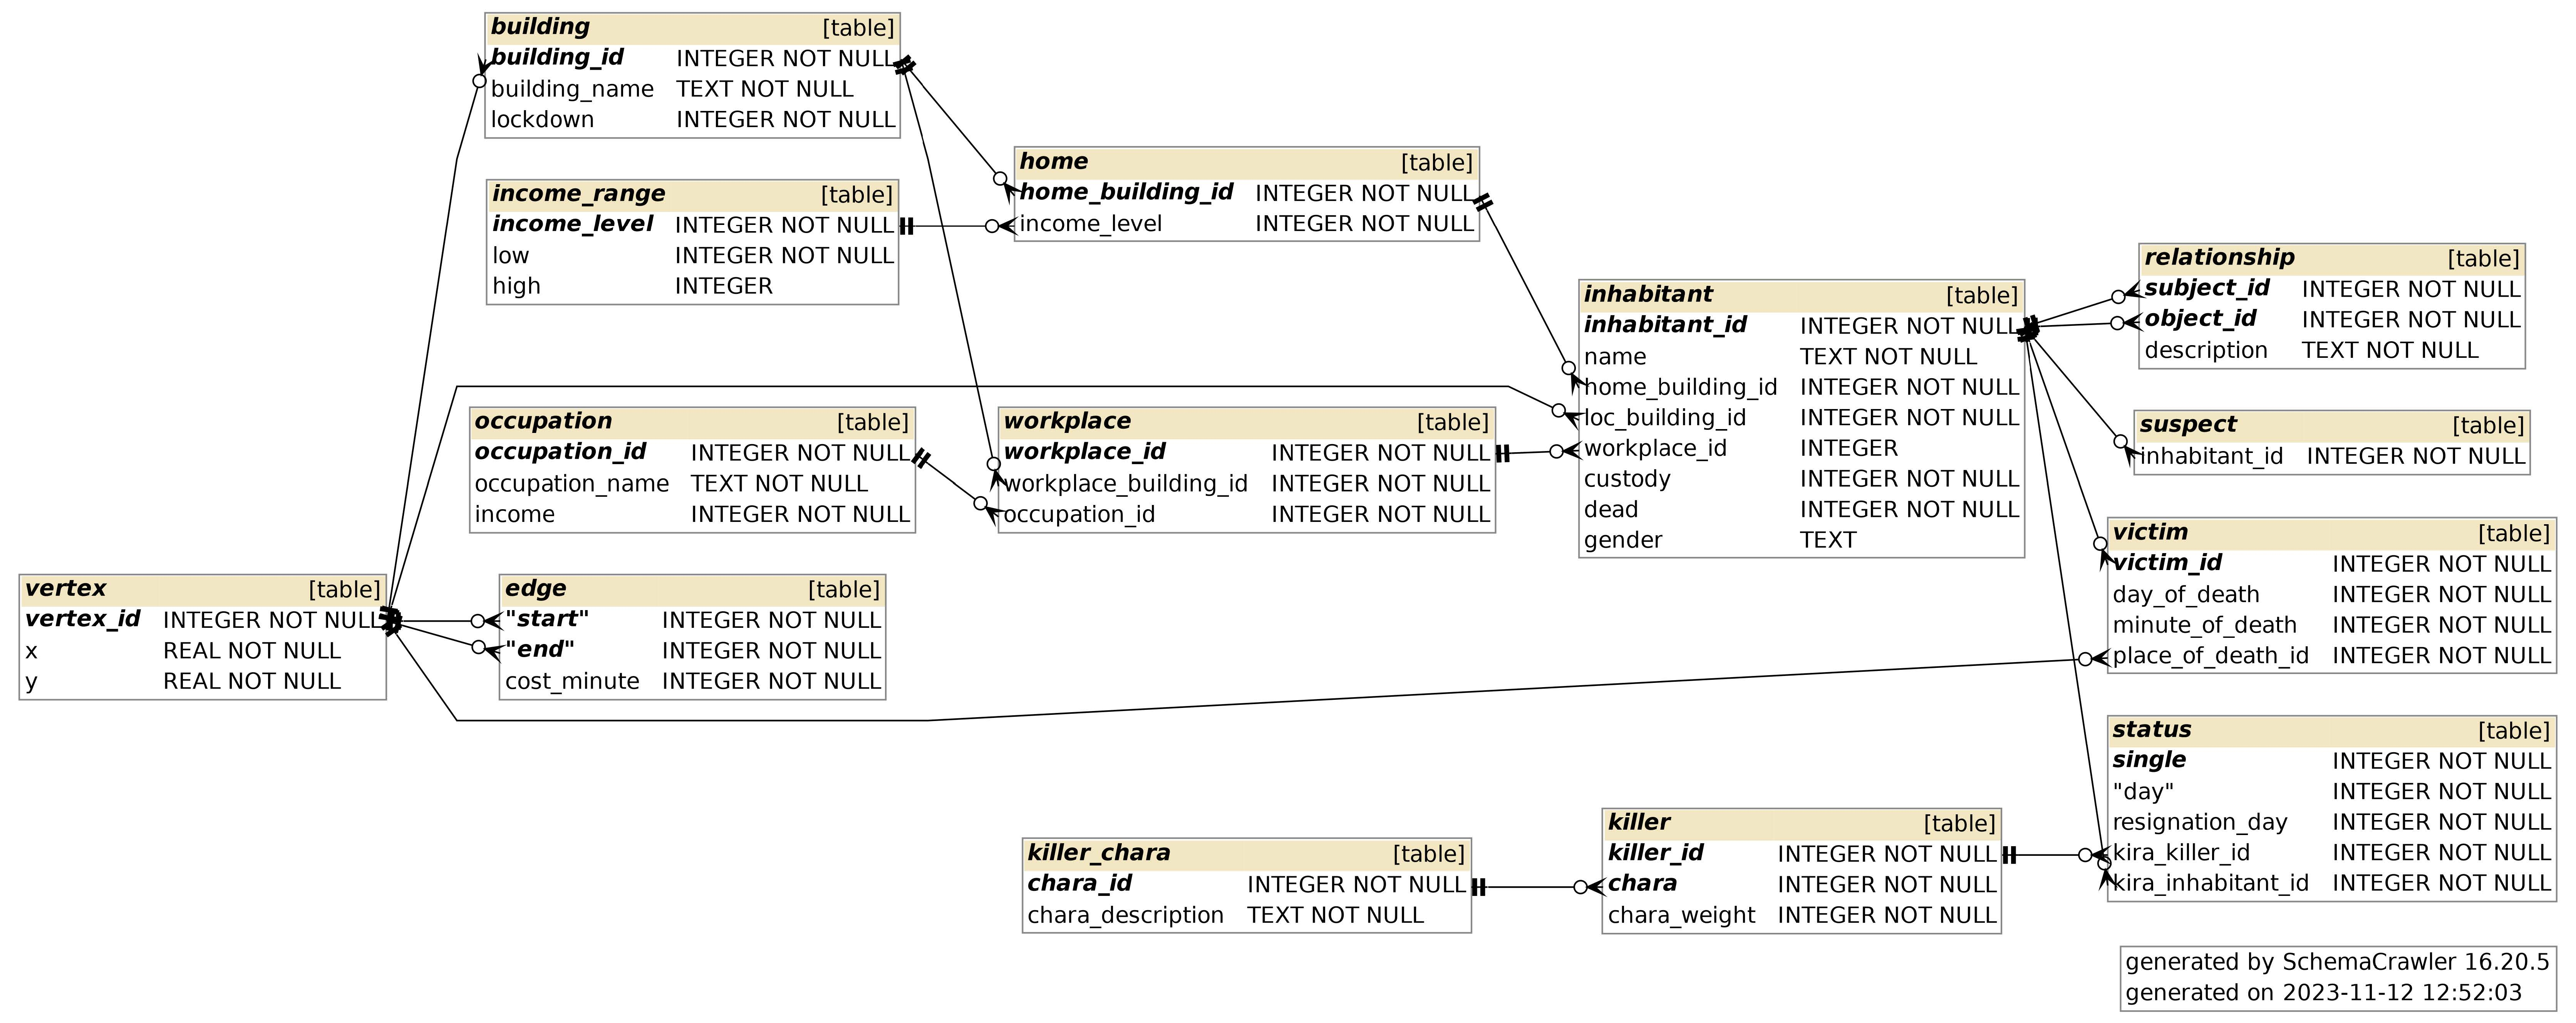
\includegraphics[width=1\textwidth]{database_version1.jpg}
  \caption{Database Schema First Version}
  \label{fig: Schema v1}
\end{figure}

The initial iteration of the Database Schema, displayed as Figure \ref{fig: Schema v1}, was formulated during the second week, a period when our acquaintance with traditional relational modeling was still developing. The following section provide a concise overview of each relation, elucidating their intended purpose and highlighting key attributes that contribute to the structural foundation of the database. This exploration aims to offer a clear understanding of the schema's components and their roles within the broader context of the simulation.

\subsubsection{\textit{inhabitant}}
The linchpin of the schema, the \textit{inhabitant} relation, serves as the cornerstone around which most other relations orbit. This table encapsulates vital characteristics defining the inhabitants in the simulation, encompassing both potential victims and perpetrators, the killers.

\begin{itemize}
    \item \textit{inhabitant\_id}: A primary key crucial for distinguishing each inhabitant uniquely.
    \item \textit{name}: The first and last name of the inhabitant, providing individual identity.
    \item \textit{home\_building\_id}: Denotes the building where the inhabitant resides or commences each day.
    \item \textit{loc\_building\_id}: Tracks the current location of the inhabitant as they move throughout the simulation.
    \item \textit{workplace\_id}: Indicates the occupation and the building where the inhabitant works.
    \item \textit{custody}: A boolean value signaling whether the player/user has designated this inhabitant as a suspect.
    \item \textit{dead}: A boolean indicator of the inhabitant's vital status, specifying whether they are deceased.
    \item \textit{gender}: Specifies the gender of the inhabitant, adding a demographic dimension to their profile.
\end{itemize}

\subsubsection{\textit{relationship}}
This table specifies the relationships between two inhabitants.

\begin{itemize}
    \item \textit{subject\_id}: Subject of the relation.
    \item \textit{object\_id}: Object of the relation.
    \item \textit{description}: The description of what the relationship is, i.g. if the description is Friend, this means object in this relationship is the friend of the subject.
\end{itemize}

\subsubsection{\textit{suspect}}
This is a list of inhabitants the user has marked to be a suspect of the murders.

\begin{itemize}
    \item \textit{inhabitant\_id}: the id of the inhabitant.
\end{itemize}

\subsubsection{\textit{victim}}
This table specifies conditions of the deaths.

\begin{itemize}
    \item \textit{victim\_id}: ID of the victim.
    \item \textit{day\_of\_death}: The day when the victim died.
    \item \textit{min\_of\_death}: The minute when the victim died.
    \item \textit{place\_of\_death\_id}: The vertex where the victim died.
\end{itemize}

\subsubsection{\textit{killer}}
This table specifies the characteristics that a killer holds.

\begin{itemize}
    \item \textit{killer\_id}: Primary key distinguishing each killer.
    \item \textit{chara}: Multi-valued attribute indicating the characteristics that a killer holds, references \textit{killer\_chara} table to display the details of the characteristic.
    \item \textit{weight}: Multi-valued attribute indicating the weight of the characteristic, i.e. the higher the weight for an attribute, the more priority the killer gives it.
\end{itemize}

\subsubsection{\textit{killer\_chara}}
This table provides description for every available killer characteristic.

\begin{itemize}
    \item \textit{chara\_id}: Primary key distinguishing each characteristic.
    \item \textit{chara\_description}: The discription of the characteristic, i.g. a characteristic may be 'low income,' this means the killer holding this characteristic has a tendency to target low income populations (depends on the weight from \textit{killer} table).
\end{itemize}

\subsubsection{\textit{vertex}}
This table identifies the locations in which inhabitants move in the simulation.

\begin{itemize}
    \item \textit{vertex\_id}: Primary key identifying each vertex in the simulation.
    \item \textit{x}: X coordinate of the vertex.
    \item \textit{y}: Y coordinate of the vertex.
\end{itemize}

\subsubsection{\textit{edge}}
This table represents the weighted and directed connections, or, roads between vertices.

\begin{itemize}
    \item \textit{start}: The vertex forming the beginning of the edge.
    \item \textit{end}: The vertex specifying the end of the edge.
    \item \textit{cost\_minute}: An indication of distance/how long it takes to travel through this edge.
\end{itemize}

\subsubsection{\textit{building}}
This table lists the important vertices in the simulation, buildings are vertices that act as destinations and sources in the path that an inhabitant takes every day.

\begin{itemize}
    \item \textit{building\_id}: Primary key distinguishing each building, this key also references the \textit{vertex\_id} in the \textit{vertex} relation, i.e., buildings are a subset of vertices.
    \item \textit{building\_name}: The name of the building.
    \item \textit{lockdown}: indication of whether the user have imposed a lockdown on the building, a building under lockdown means it no longer can be a part of a path nor can it become the designation of all inhabitants.
\end{itemize}

\subsubsection{\textit{occupation}}
This table specifies the available occupations that inhabitants can have.

\begin{itemize}
    \item \textit{occupation\_id}: Primary key distinguishing each occupation.
    \item \textit{occupation\_name}: The name of the occupation.
    \item \textit{income}: The income of the inhabitant who has the occupation, there is an implicit reference to the \textit{income\_range} table which shall be explained later.
\end{itemize}

\subsubsection{\textit{workplace}}
This table identifies the workplace of an inhabitant, that is, the building where an inhabitant goes to work. A workplace building can host up to three different occupations

\begin{itemize}
    \item \textit{workplace\_id}: Primary key distinguishing each workplace.
    \item \textit{workplace\_building\_id}: The vertex/location of the workplace.
    \item \textit{occupation\_id}: One of the occupations in the workplace.
\end{itemize}

\subsubsection{\textit{income\_range}}
This table specifies an inhabitant's wealth status based on the income provided by the Occupation table.

\begin{itemize}
    \item \textit{income\_level}: The level of income, every inhabitant is categorized to 'low income,' 'medium income,' or 'high income.'
    \item \textit{low}: Attribute specifying the low range (inclusive) of the income level.
    \item \textit{high}: Attribute specifying the high range (inclusive) of the income level, using null to denote positive infinity.
\end{itemize}

\subsubsection{\textit{home}}
This table specifies the home of the inhabitants, each home is a building in the vertex map.

\begin{itemize}
    \item \textit{home\_building\_id}: Primary key distinguishing each home. This is also a reference to the \textit{building} relation.
    \item \textit{income\_level}: Each inhabitant is assigned to a home based on their income level, which in turn is based on their occupation.
\end{itemize}

\subsubsection{\textit{status}}
This table specifies the progress of the simulation, information that needs to be kept for the purpose of loading and saving a simulation instance.

\begin{itemize}
    \item \textit{single}: Specifying that there is can be only one tuple in this relation. It is constrained so that it must have the default value of 0 and that it is also the primary key.
    \item \textit{day}: How many ``days" have passed in this simulation.
    \item \textit{resignation\_day}: When the user will ``resign" in the simulation. When the \textit{regisnation\_day} equals the day attribute, this is when the simulation ends, signalling a failure to identify the killer.
    \item \textit{kira\_killer\_id}: Selects a killer in the \textit{killer} table.
    \item \textit{kira\_inhabitant\_id}: Matches the killer with an identity in \textit{inhabitant}.
\end{itemize}

\subsection{The ER Model}
\begin{figure}
  \centering
  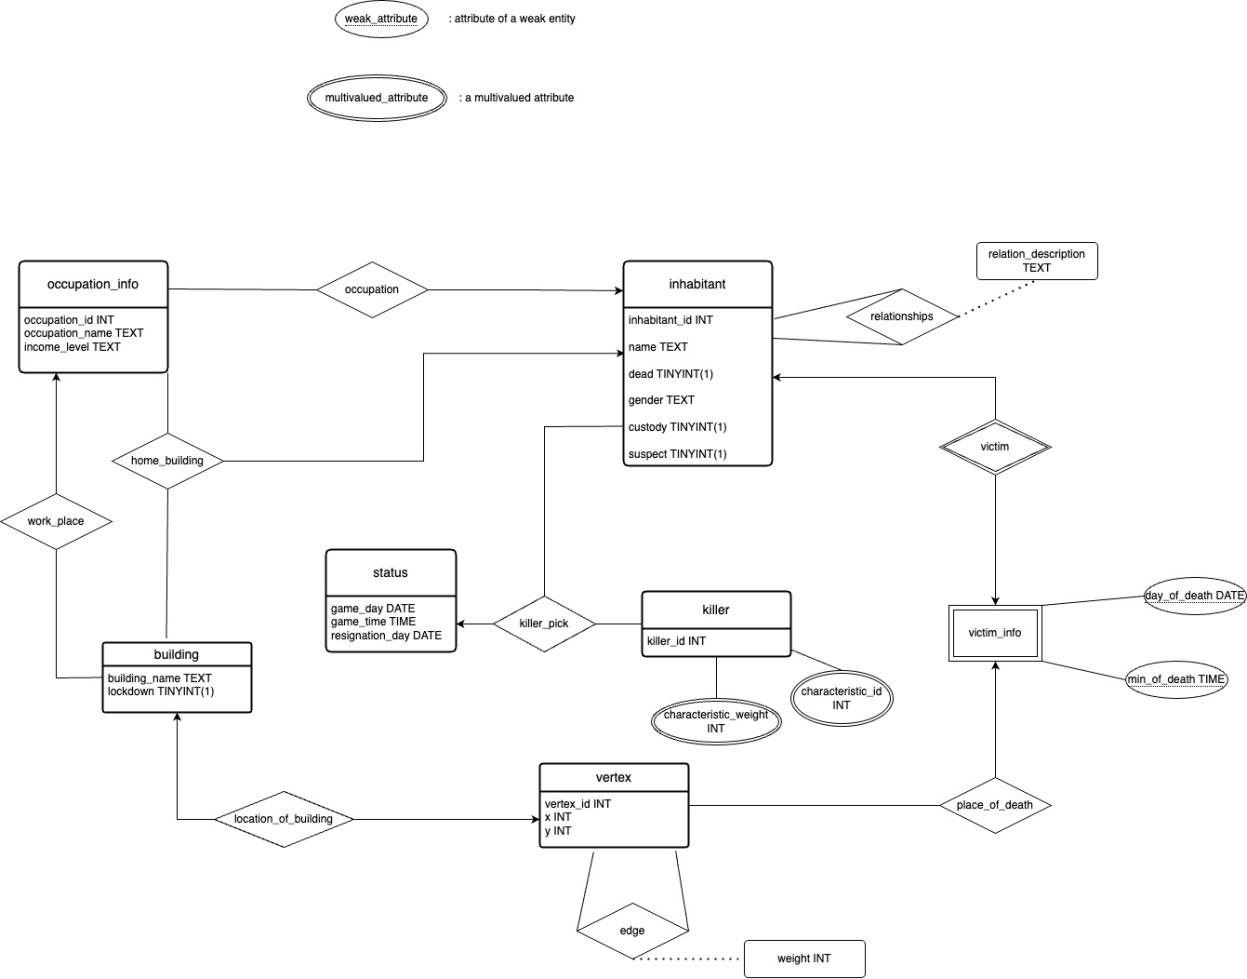
\includegraphics[width=1\textwidth]{ER_model.jpg}
  \caption{ER model in the fifth week}
  \label{fig: ER Model}
\end{figure}
Figure \ref{fig: ER Model} illustrates the Entity-Relationship (ER) model crafted during the fifth week of the course. During the refinement process, redundant attributes were systematically removed, streamlining the model for enhanced clarity and efficiency. Noteworthy adjustments were made to certain attributes, such as the \textit{killer} table, where a redesign rendered its attributes multi-valued. This modification aligns with conventional ER model design principles. While a relational model have been converted from this ER model, it was ultimately not used as the final database design. The final schema, however, did incorporate some changes made in the ER model, the following section highlights some of these changes.

\subsection{The Final Version}
\begin{figure}
  \centering
  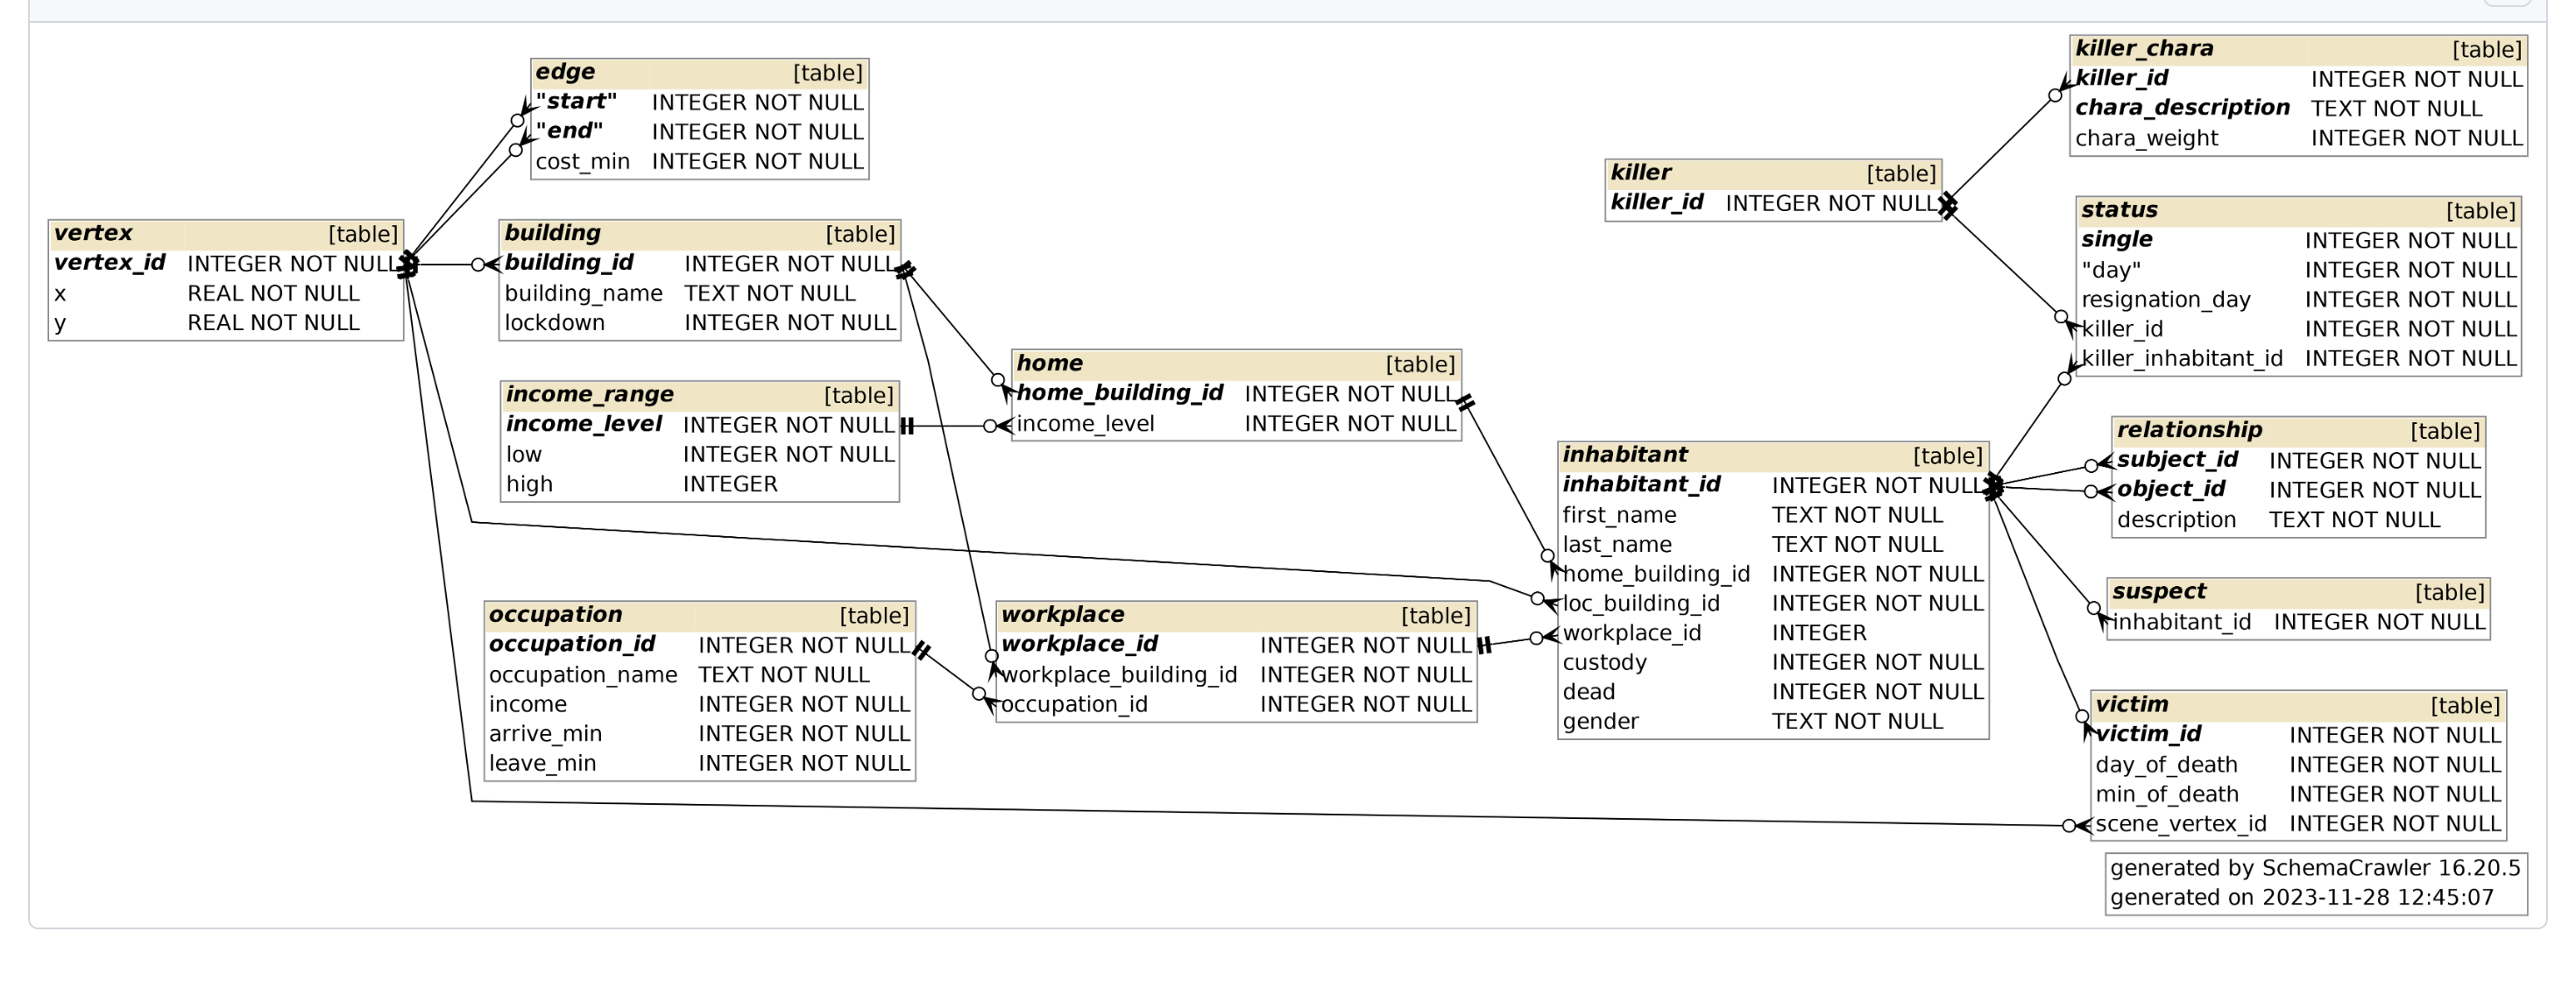
\includegraphics[width=1\textwidth]{Final_Database_Schema.png}
  \caption{ER model in the fifth week}
  \label{fig: Final Database Schema}
\end{figure}
The Final Database Schema is presented in Figure \ref{fig: Final Database Schema}. This changes made to form this version of the schema reflected several issues that were not considered in the initial schema.

\subsubsection{Key Changes}
\paragraph{\textit{inhabitant}}
Separation of \textit{name} to atomic components first and last names. This change was made to make build relationships between inhabitants via the \textit{relationship} table. One challenge faced in the generation of test dataset was the formation of resonable relationships between inhabitants. With the separation into first and last name, inhabitants with the same last name can be easily placed in \textit{relationship} to be ``relatives".

\paragraph{\textit{killer and killer\_chara}}
\textit{killer} and \textit{killer\_chara} is entirely redesigned. Originally the \textit{killer\_id} and \textit{chara} attribute formed the primary key of table \textit{killer}, this eventually proved to be an issue in the implementation of several queries including Victim Selection; this is because many tables needed to form a foreign key reference with the \textit{killer\_id} attribute in the \textit{killer} table. This problem was address by having the \textit{killer\_id} isolated to form the killer table on its own, \textit{killer\_chara} is then moved to \textit{killer\_chara} to form an ``id-characteristic" pair that uniquely identifies a characteristic of a killer.

\paragraph{\textit{occupation}}
Two attributes, \textit{arrive\_min} and \textit{leave\_min} were added to the \textit{occupation} table in order to add uniqueness to an inhabitant's trajectory in a day.

\section{Important Queries and Implementations}
\subsection{Path Finding and Generation}
The path generation query serves a pivotal role in the simulation by generating a temporary table that captures the movements of all inhabitants during a round. Executed at the initiation of each new round, this query stands as one of the most crucial operations in the simulation. Its significance lies in introducing randomness to the actions of both inhabitants and the killer. The killer's modus operandi heavily depends on the paths taken by both the inhabitants and themselves each day. The intricacies of the killing mechanism hinge on the precise intersection of paths, as a killer can only perpetrate a murder when an inhabitant's and the killer's trajectories coincide at the same period.

Path generation is divided to two steps: calculation of the shortest path using Dijkstra's all pairs shortest path and generating a viable path for the inhabitant using information from the shortest path. Both steps are implemented recursively using triggers due to that stored function/stored procedure is not supported by SQLite. Since SQLite is executed in the same process as the application, there would be no performance benefits in using stored function/stored procedure compared to a client-server setup where the stored code could be run in the server side as opposed to the client side.

\subsubsection{All Pairs Shortest Path Algorithm Via Dijkstra's Algorithm}
The \textit{dist} table as shown in Listing \ref{lst:dist} stores the shortest distance from \textit{src} to \textit{dst} in \textit{d}. The \textit{visited} attribute is a boolean variable that is set to true when the \textit{dst} vertex is added to the set of visited vertices starting from \textit{src} as described in Dijkstra's algorithm.\cite{dijkstra_wikipedia} A visited set is maintained for each \textit{src}, which indicates that the shortest distance from \textit{src} to these vertices are known.

\begin{listing}[H]
    \inputminted[firstline=24, lastline=30, breaklines=true]
    {sql}{shortest_path.sql}
    \caption{The \textit{dist} table.}
    \label{lst:dist}
\end{listing}

Dijkstra's algorithm is implemented as a recursive trigger.\cite{sqlite_forum}. Initially, the distance between all pairs of vertices are null as shown in Listing \ref{lst:shortest_path_init}. The distance between each vertex and itself is then set to 0 and each source vertex is added to the visited set starting from itself. By updating the \textit{visited} attribute of each source vertex, the trigger is fired.

\begin{listing}[H]
    \inputminted[firstline=52, lastline=60, breaklines=true]
    {sql}{shortest_path.sql}
    \caption{The initial insertion of null distance pairs and updating distances from each vertex to themselves to 0.}
    \label{lst:shortest_path_init}
\end{listing}

During each execution of the trigger shown in Listing \ref{lst:shortest_path}, the known shortest distances and the visited set starting from \textit{NEW.src} are updated. Firstly, the sums of the distance between \textit{NEW.src} and \textit{NEW.dst} plus the edge cost from \textit{NEW.dst} to to the adjacent vertices are used to update the shortest distances to these adjacent vertices. Then, the unvisited vertex that is the closest to \textit{NEW.src} is added to the visited set. This then fires the trigger recursively.

\begin{listing}[H]
    \inputminted[firstline=34, lastline=50, breaklines=true]
    {sql}{shortest_path.sql}
    \caption{Dijkstra's algorithm implemented using a recursive trigger.}
    \label{lst:shortest_path}
\end{listing}

\subsubsection{Path Generation}

A inhabitant's daily path could be described by location-time pairs, indicating that they are at a specific vertex for a specific period time of their day. Their path is constrained by their daily routine, such as when they get up, when they must be at work, when they could leave work, and when they must be at home. The \textit{src\_dst} table shown in Listing \ref{lst:src_dst} describes such constraints, specifying that the inhabitant with \textit{inhabitant\_id}, they may leave \textit{src} no earlier than \textit{t\_src} and must arrive at \textit{dst} no later than \textit{t\_dst}. For each inhabitant with a job, their daily routine could be described with two tuples in the \textit{src\_dst} table. One constraining the time they go from home to work, and the other constraining the opposite.

\begin{listing}[H]
    \inputminted[firstline=17, lastline=24, breaklines=true]
    {sql}{init_loc_time.sql}
    \caption{The \textit{src\_dst} table.}
    \label{lst:src_dst}
\end{listing}

The resulting path in location-time pairs is stored in the \textit{loc\_time} table shown in Listing \ref{lst:loc_time}. Each tuple describes that the inhabitant with \textit{inhabitant\_id} will arrive at \textit{vertex\_id} on the minute of \textit{arrive} attribute and leave on the minute of \textit{leave} attribute. The \textit{dst} and \textit{t\_dst} attributes are the same as those two attributes in \textit{src\_dst} for convenience.

\begin{listing}[H]
    \inputminted[firstline=28, lastline=38, breaklines=true]
    {sql}{init_loc_time.sql}
    \caption{The \textit{loc\_time} table.}
    \label{lst:loc_time}
\end{listing}

The daily path of an inhabitant is generated by randomly walking from \textit{src} to \textit{dst} while satisfying the constraints. This is implemented using a recursive trigger. Initially, the inhabitant waits at the source vertex for some random time limited by the fact that they must be able to at least reach the destination on time taking the shortest path. These initial location-time pairs are then inserted into \textit{loc\_time} as shown in Listing \ref{lst:path_generation_init}.

\begin{listing}[H]
    \inputminted[firstline=3, lastline=9, breaklines=true]
    {sql}{query_loc_time.sql}
    \caption{Insertion of initial location-time pairs.}
    \label{lst:path_generation_init}
\end{listing}

Inserting the initial conditions fires the trigger shown in Listing \ref{lst:path_generation} recursively. For each tuple inserted into \textit{loc\_time} where the destination is not reached, a neighboring vertex is randomly selected to be the next vertex that the inhabitant advances to. This vertex, however, has to satisfy the condition that the current time, plus the time cost of going to that vertex, and plus the shortest distance of going from that vertex to the destination does not exceed \textit{t\_dst}. A random portion of the time available to spare after taking all these into account is then chosen to be the duration that the inhabitant waits at the neighboring vertex. The new location-time pair is then also inserted into the table.

\begin{listing}[H]
    \inputminted[firstline=42, lastline=63, breaklines=true]
    {sql}{init_loc_time.sql}
    \caption{Path generation implemented using a recursive trigger.}
    \label{lst:path_generation}
\end{listing}

\subsection{Victim Selection}
The Victim Selection script performs the crucial task of choosing a victim for the killer when executed. This script follows the execution of the previously explained path generator. The selection process considers multiple factors. Foremost among these is the intersection of paths between the killer and potential victims, a pivotal element in determining the feasibility of a murder. Additionally, the script accounts for the killer's proclivity to target specific segments of the population, as specified in the \textit{killer\_chara} table. By integrating these considerations, the script not only adds an element of realism to the simulation but also introduces a layer of complexity that aligns with the characteristics and tendencies attributed to the killer in the simulation environment.

The script presented in Listing \ref{lst:victim_selection} is designed to construct two temporary tables, namely \textit{pot\_victim} and \textit{weighed\_pot\_victim}. The former serves as a representation of potential victims, while the latter refines this selection by sorting potential victims based on their weight, determined by the killer's characteristics. The \textit{pot\_victim} table contains information on inhabitants deemed viable targets for the killer – those with intersecting paths on the given \textit{day} of the simulation. The population of this table involves a query that assesses inhabitants sharing a vertex with the killer at the same time. The utilization of the max and min functions tracks overlapping time intervals, subsequently facilitating the generation of a time of death.

The initialization of \textit{weighed\_pot\_victim} is done through a joining of pertinent tables, incorporating information for weight determination, including details from the Home and Workplace tables. The inclusion of the \textit{killer\_chara} table facilitates the assignment of weights based on the distinct characteristics of the killer. Within the \textbf{WHERE} clause, a \textbf{CASE} statement dynamically evaluates the characteristics fulfilled by each inhabitant. The subsequent \textbf{SELECT} clause projects pairs of inhabitants and their respective characteristics, accompanied by the corresponding weights extracted from the \textit{killer\_chara} table.

Afterwards, \textit{weighed\_pot\_victim} is used in the final query that groups each inhabitant by their id and have their total weight calculated using an aggregate function. The inhabitant is sorted by descending order based on the calculated weight with information summarized in the \textbf{SELECT} clause, the time of death is calculated by randomly selecting a period from the overlapping time interval calculated from \textit{pot\_victim}. Using this final query, the victim is chosen by fetching the first tuple from python.

\begin{listing}[H]
    \inputminted[firstline=3, lastline=36, breaklines=true]
    {sql}{kill_sequence.sql}
    \caption{Victim Selection script.}
    \label{lst:victim_selection}
\end{listing}

\begin{listing}[H]
    \ContinuedFloat
    \inputminted[firstline=37, breaklines=true]
    {sql}{kill_sequence.sql}
    \caption{Victim Selection script.}
    \label{lst:victim_selection}
\end{listing}

\subsection{Witness Count}

The Witness Count query counts the number of times each inhabitant has been witnessed on a certain vertex. It aims at reflecting that in many detective novels, the police can put up posters asking the general public about whether they have seen suspicious people in certain places. Our implementation is a bit naive as it simply counts the number of witnesses regardless of the ``suspiciousness".

As shown in Listing \ref{lst:witness_count}, the query counts the number of times that the a given inhabitant \textit{a} has being on the same vertex as as any inhabitant (witness) \textit{b} at the same time. It checks for temporal overlaps by comparing the time that \textit{a} and \textit{b} have arrived and left the given vertex. Simultaneously, the inhabitant \textit{a} must not be dead before reaching the given vertex and that the witness \textit{b} must be alive at the end of the turn to tell the tale.

\begin{listing}[H]
\inputminted[breaklines=true]{sql}{witness_count.sql}
\caption{Witness Count query.}
    \label{lst:witness_count}
\end{listing}

\subsection{Victim Commonality}
The \textit{commonality} view is a perspective that reveals recurring patterns among the victims within a particular simulation instance. This query extracts and presents attributes along with their corresponding values that have manifested across multiple victims. The significance of this view lies in its ability to succinctly summarize information about the victims throughout the simulation. Consequently, it plays a pivotal role in the profiling of the killer. This functionality proves indispensable not only in the context of the simulation but also mirrors its critical counterpart in real-world scenarios, emphasizing its role in enhancing the understanding and analysis of patterns in criminal cases.

The query is written to be a view because it will be frequently updated and accessed, in every round of the simulation.

Listing \ref{lst:victim_commonality} presents the definition of the view. Initially, a local query table named victim\_info is created using the WITH clause. This table proves instrumental in subsequent subqueries and is, therefore, invoked within the WITH clause. The ensuing query employs a subquery named 'attributes' within the FROM clause. 'Attributes' encapsulates a collection of victim information attributes extracted from victim\_info and projects them in the format of name and value pairs. This operation essentially assembles tuples for each victim alongside their respective attributes. Notably, the process necessitates the use of UNION to concatenate diverse attributes that must be considered, ensuring a comprehensive dataset. Additionally, attributes not of datatype TEXT are explicitly cast to align with the specified schema. After 'attributes' is queried, it is grouped by the name and value pairs and filtered to include only pairs that recurred at least thrice, the pair is then projected by the SELECT clause along with the recurrence and sorted by descending order.

\begin{listing}[H]
    \inputminted[breaklines=true]{sql}{victim_common_attribute.sql}
    \caption{Victim commonality view.}
    \label{lst:victim_commonality}
\end{listing}

\section{Simulation Demo}

The following is a minimal user interface created using DearPyGui.\cite{dearpygui_github}

\subsection{Main Menu} 
Figure \ref{fig:main_menu} presents the Main Menu of the simulator, the user has three options: start a new game, load a saved game, and quit the simulator.

\begin{figure}[H]
  \centering
  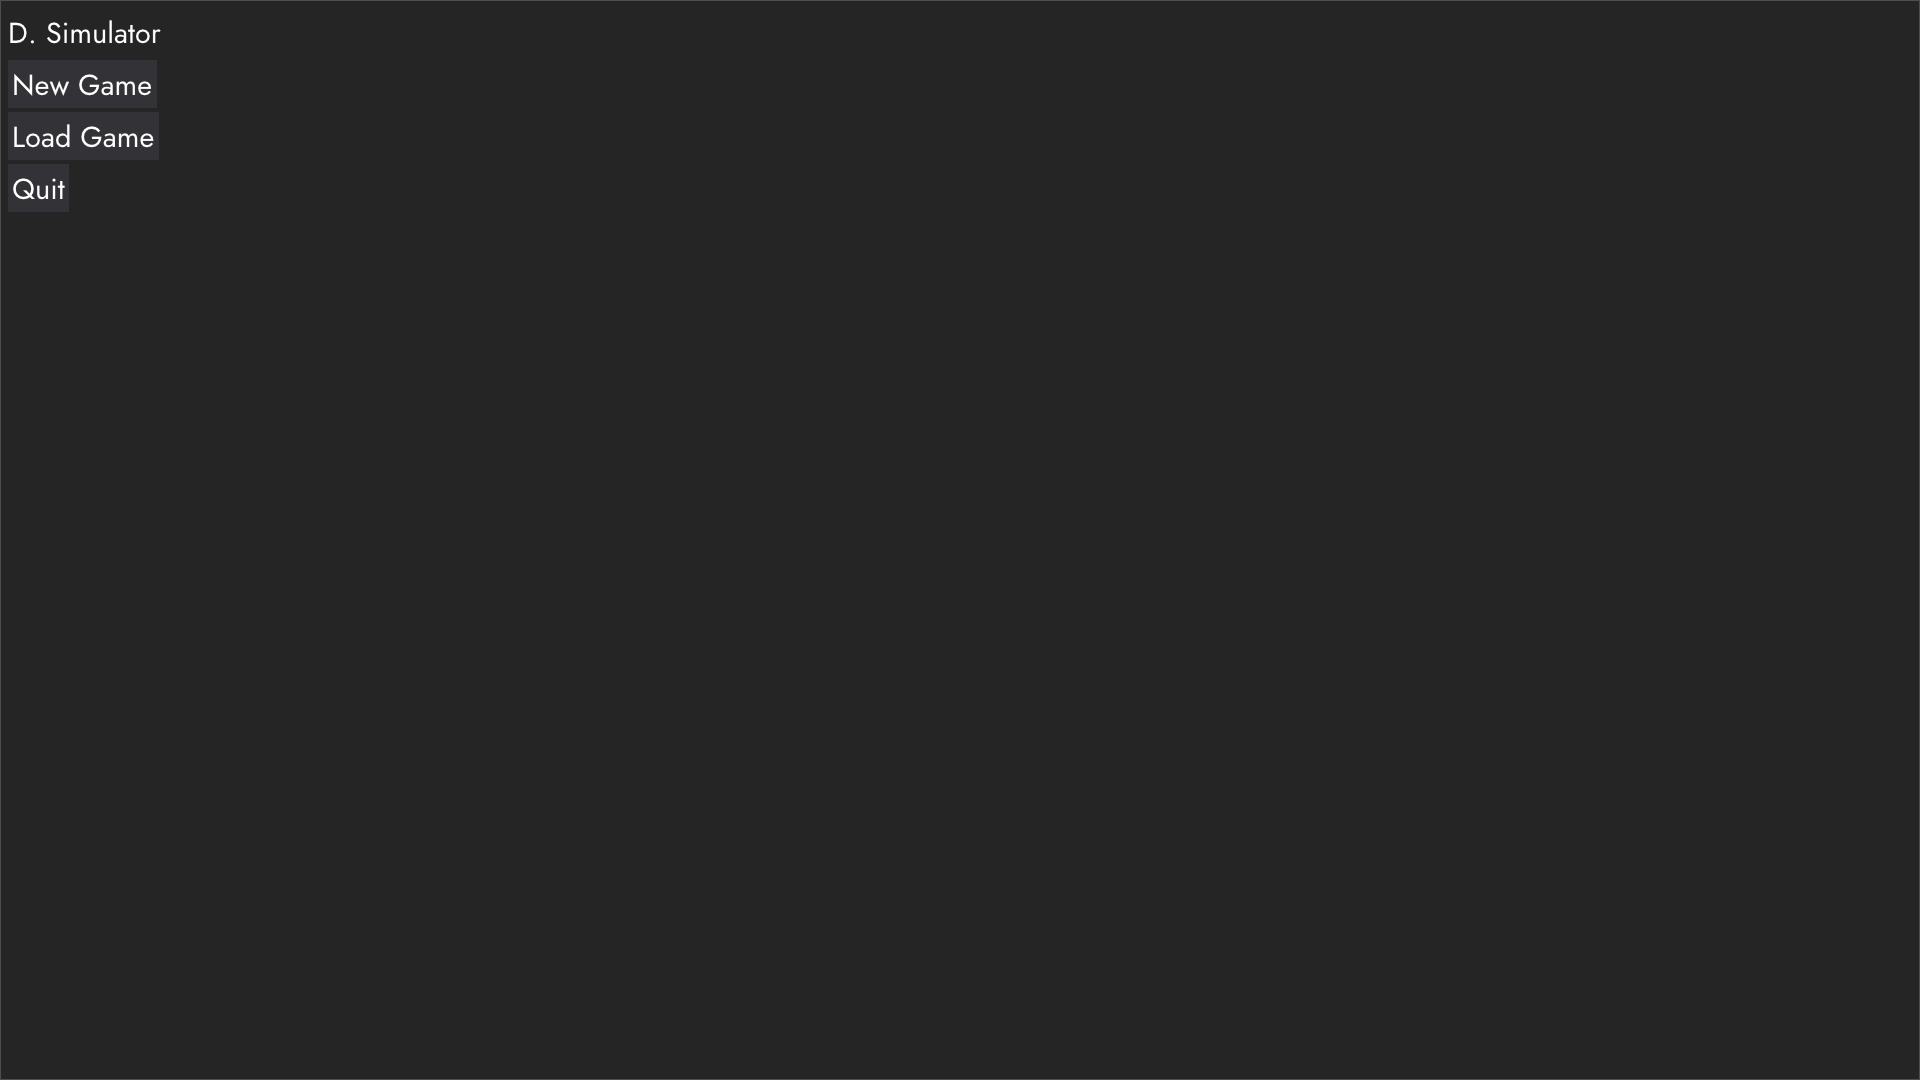
\includegraphics[width=1\textwidth]{main_menu.png}
  \caption{Main Menu.}
  \label{fig:main_menu}
\end{figure}

\subsection{Load Screen}
In figure \ref{fig:load_game} the Load Screen is presented, here the user can find previously saved games. The user has the ability to load a saved game or delete it.

\begin{figure}[H]
  \centering
  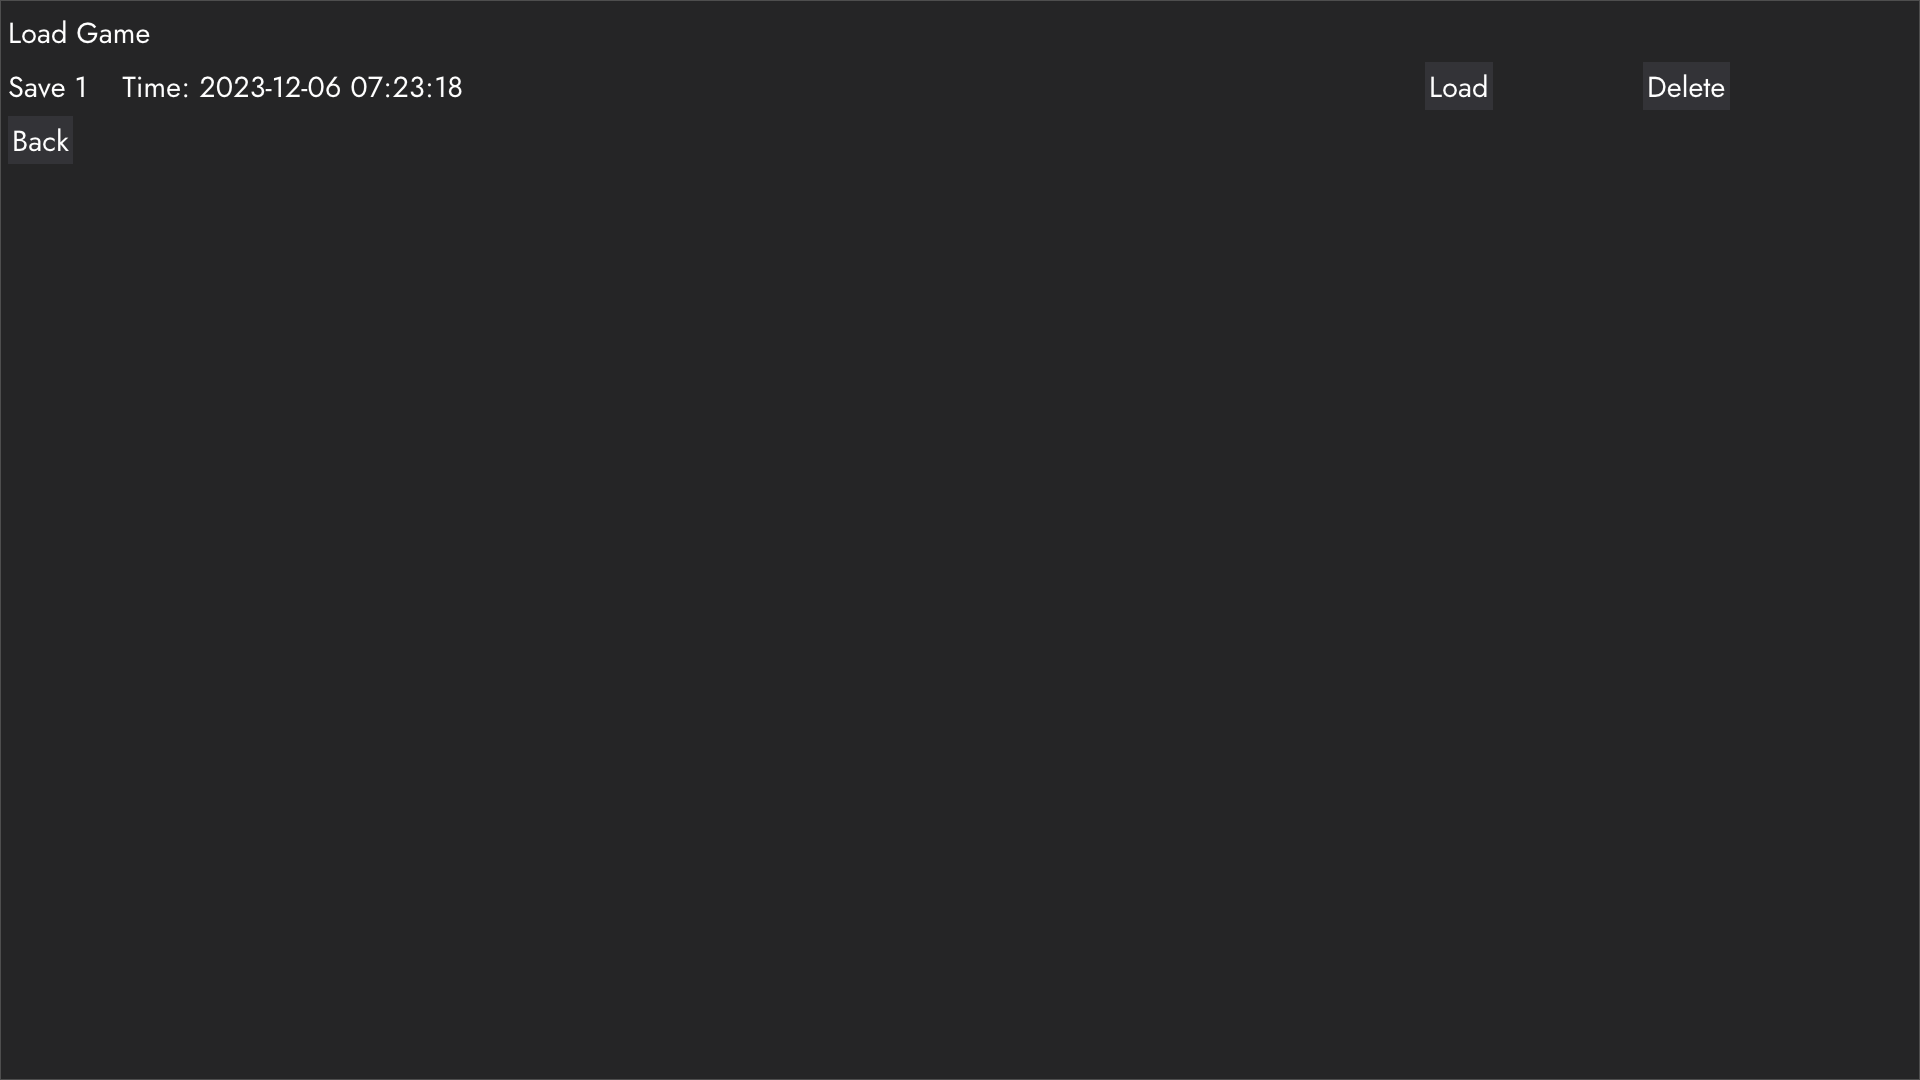
\includegraphics[width=1\textwidth]{load_game.png}
  \caption{Load Screen.}
  \label{fig:load_game}
\end{figure}

\subsection{Game Window}
After loading or starting a game, the user enters the Game Window, which displays a variety of information and tools as presented in Figure \ref{fig:game_window}. On the left of the screen a scrollable map is displayed. This map identifies the individual vertices as white circles, and the buildings as red squares. The white lines connecting each vertex are the edges. Every vertex is labeled by its ID, every building is labeled by its name, and every edge is labeled by its weight (\textit{cost\_min} attribute).

On the right hand side of the screen is a query box for searching inhabitants with specific attributes, the search results are on the bottom. The user is free to enter any filter information into the query box. In this case, the user searches for all inhabitants with occupation equal to ``Agricultural engineer," the query results, ``Rebecca," ``Mark," etc. are therefore the inhabitants that have the occupation ``Agricultural engineer."

\begin{figure}[H]
  \centering
  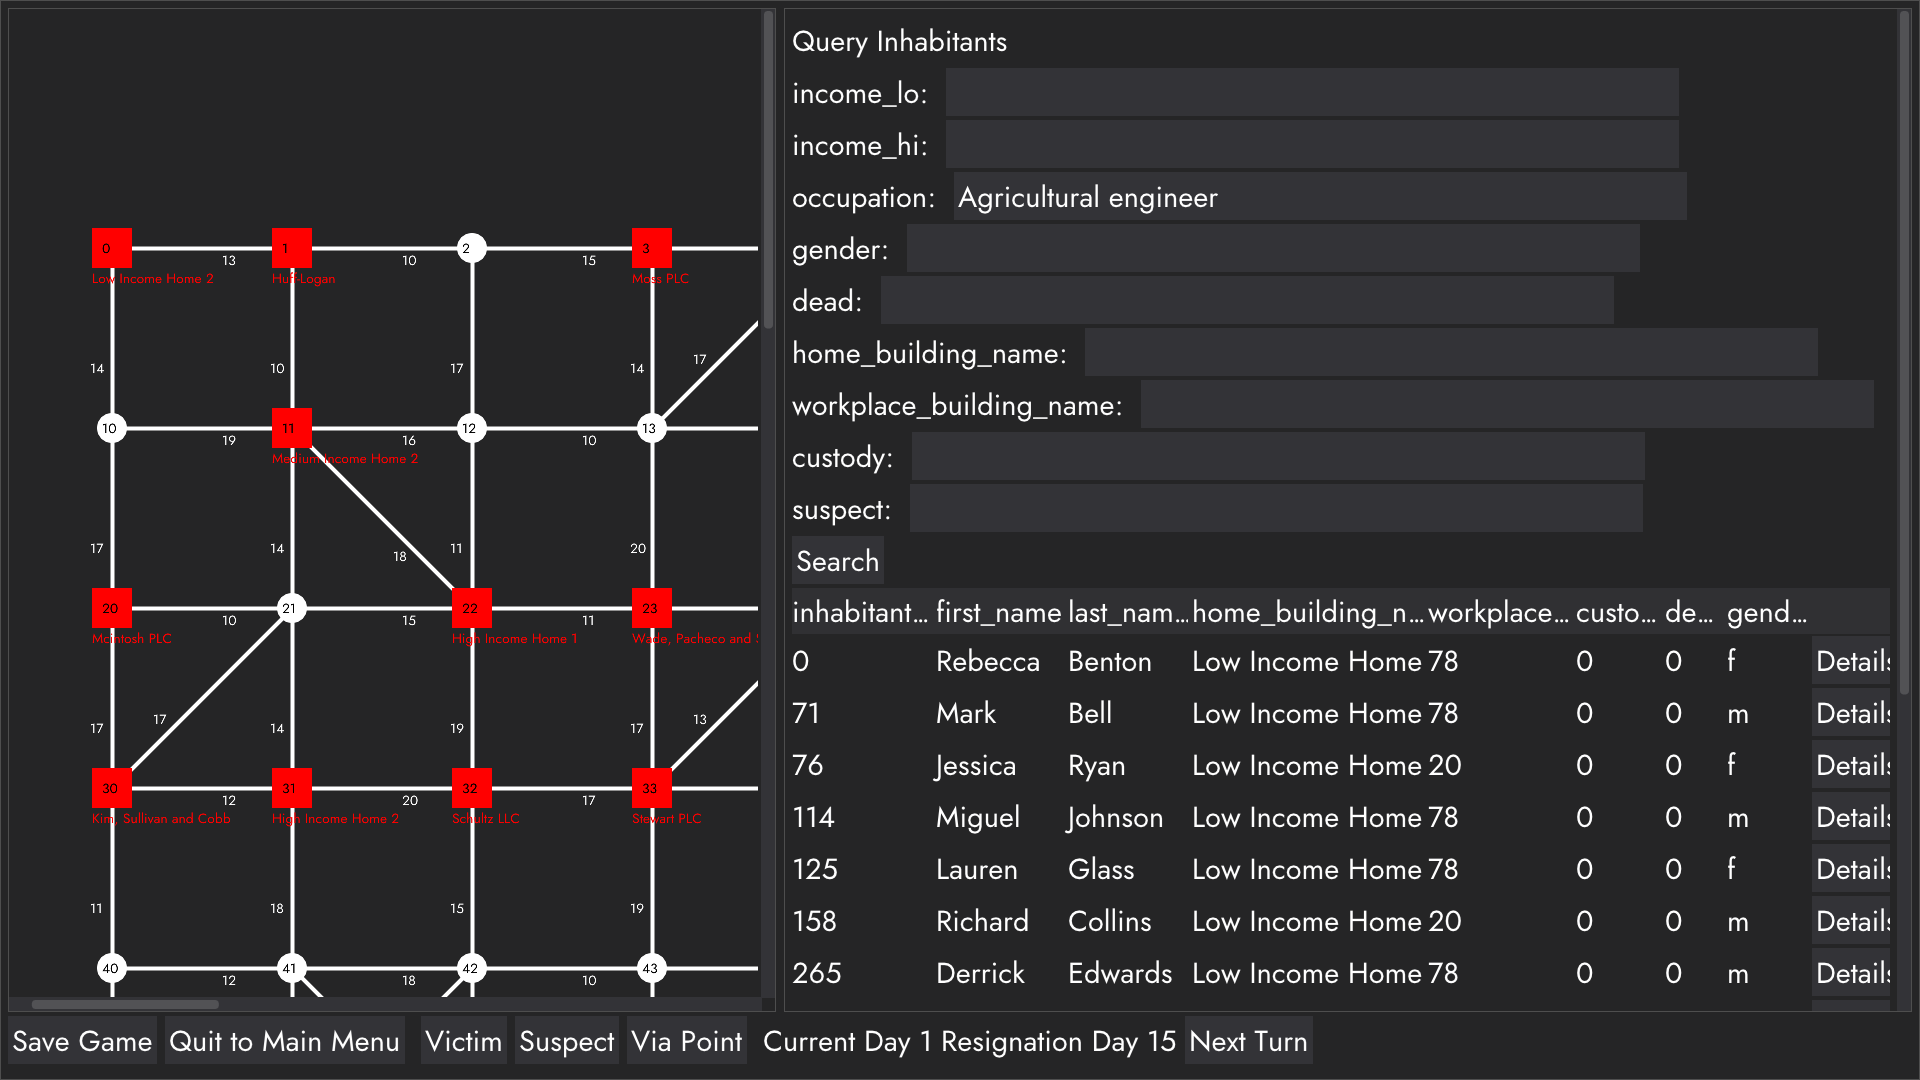
\includegraphics[width=1\textwidth]{game_window.png}
  \caption{Game Window.}
  \label{fig:game_window}
\end{figure}

\subsection{Building Detail and Inhabitant Detail}
When the buildings on the map is clicked, a screen displaying the information of the building is provided as seen on the left view of Figure \ref{fig:building_inhabitant_detail}. It displays components such as the name of the building, ``Mcintosh PLC" in this case, whether if it is under lockdown, the occupations that work in this building, and the inhabitants that visit this building. The user is capable of placing a building into lockdown using ``Toggle Lockdown," which disables all edges involving this building and thus limiting the paths of various inhabitants in the next turn.

When the user wish to view the details of an inhabitant, they can click on the ``Details" button to the right of every inhabitant tuple. When clicked, a screen on the right will pop up displaying the details of the selected inhabitant; in the case of Figure \ref{fig:building_inhabitant_detail}, we are looking at details of ``Rebecca Benton." On this screen, there are a few tools that can be used, such as ``Toggle Suspect," such sets or unsets the inhabitant as a suspect, or ``Accuse" which means this inhabitant is selected as the person the user believes is the killer, the program will provide a feedback of whether if the user has selected the correct inhabitant as the killer as shown in Figure \ref{fig:win}.

\begin{figure}[H]
  \centering
  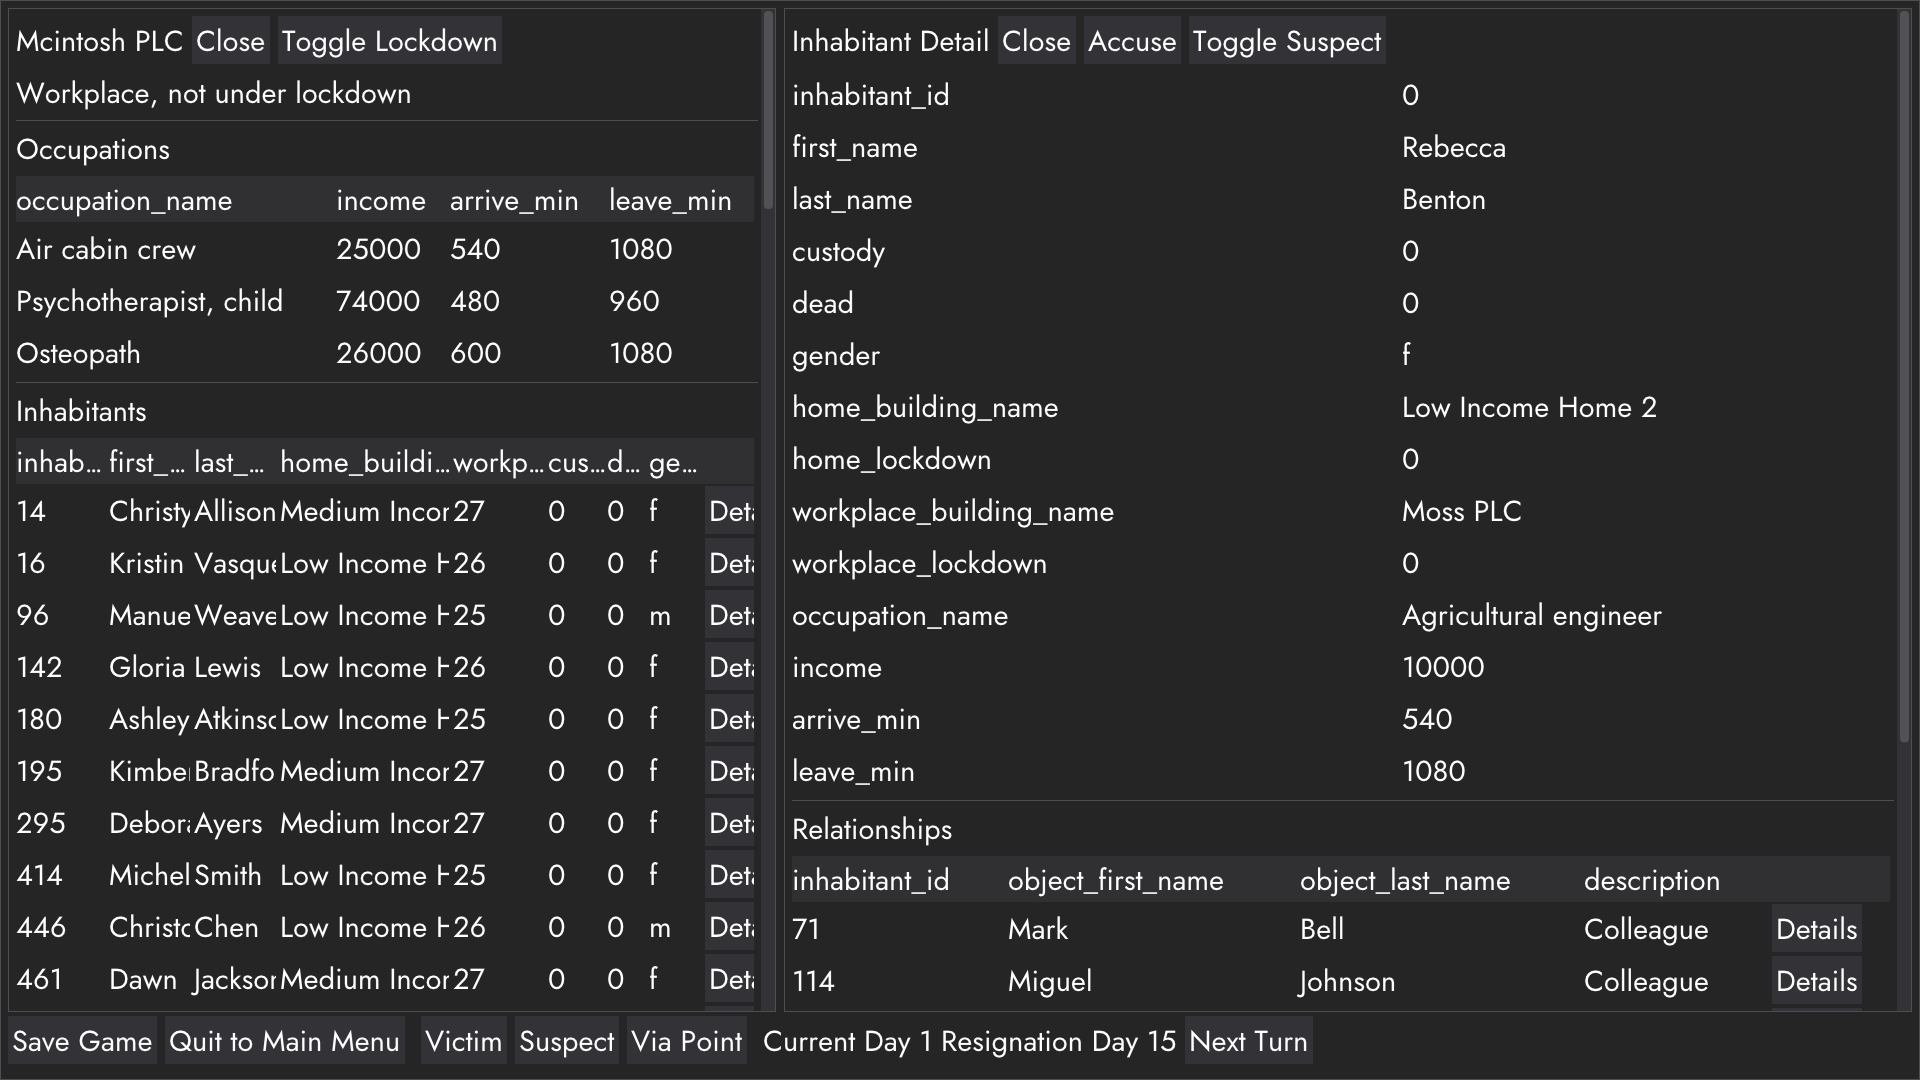
\includegraphics[width=1\textwidth]{building_inhabitant_detail.png}
  \caption{Building Detail and Inhabitant Detail.}
  \label{fig:building_inhabitant_detail}
\end{figure}

\begin{figure}[H]
  \centering
  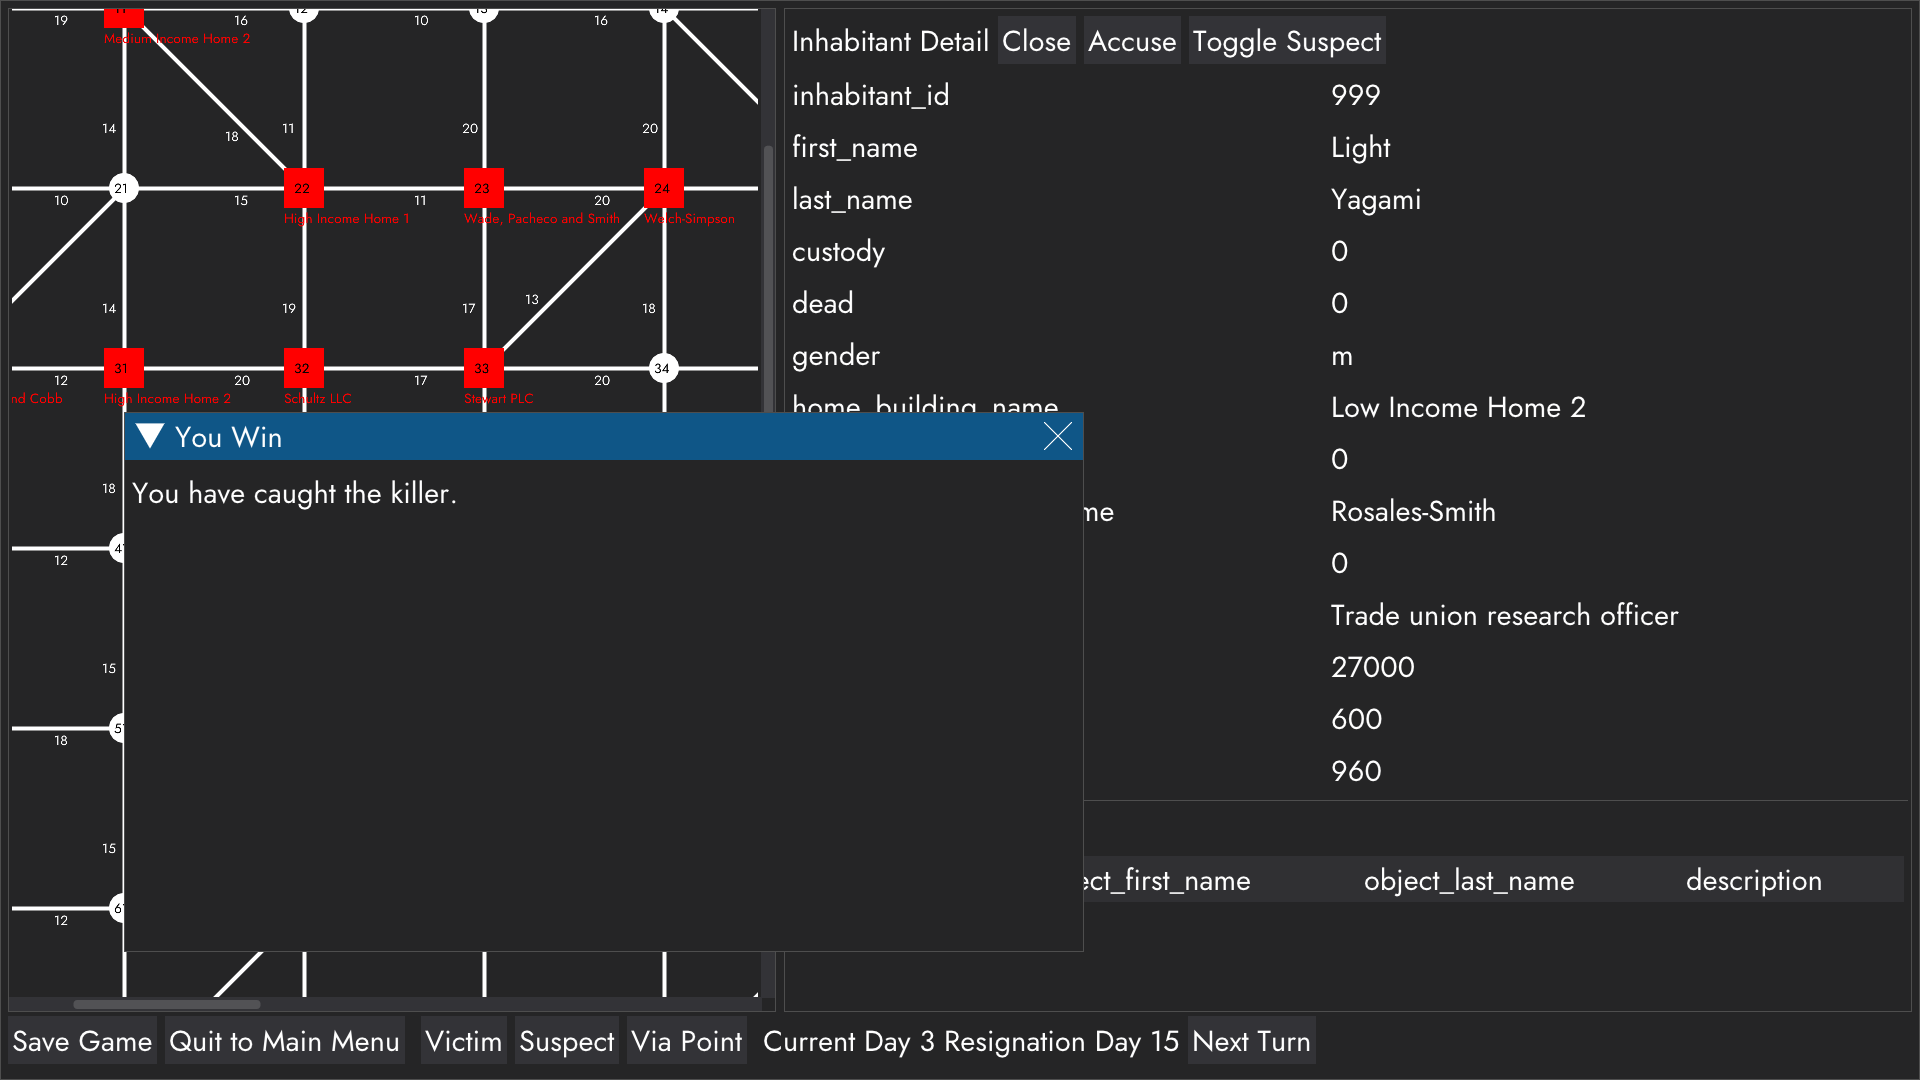
\includegraphics[width=1\textwidth]{win.png}
  \caption{Winning the game.}
  \label{fig:win}
\end{figure}

\subsection{Other Features}
The Game Window also provides several other features such as Victim Window, Suspect Window and the ``Via Point" query. When the ``Victim" button is clicked, the information on the inhabitants killed in this simulation is displayed. In Figure \ref{fig:victim_suspect_via_point}, three inhabitants are killed and the attributes shared among the three inhabitants are displayed, the table represents the name of the attribute, value of the attribute and how many times the attribute has occurred among the victims.

Clicking on ``Suspect" opens a window that displayed the information on the inhabitants placed in the suspect list, the example displayed on the top right corner of Figure \ref{fig:victim_suspect_via_point} shows the information of ``Rebecca" who is marked as a suspect by the user.

Clicking on ``Via Point" opens another window with a query box. Here, the user can enter a starting vertex, ending vertex, and a time frame. The results of the query shown in Figure \ref{fig:victim_suspect_via_point} are vertices that an inhabitant is capable of visiting in a path, given that the inhabitant starts on vertex 1, and has 60 minutes to get to vertex 10.

Relationships of an inhabitant can be seen by scrolling down in the ``Details" window of an inhabitant; on the right of Figure \ref{fig:witness_counts_relationships} shows us the relationships an inhabitant has. The ID of the ``object" is displayed along with his/her name  and a description of the relationship.

The ``Witness" information can also be found on the ``Details" window of a building. Similarly with relationship, the user has to scroll down in the Details window to find the inhabitants that were seen visiting this building in a particular turn. An example of this is also provided to the left of Figure \ref{fig:witness_counts_relationships}.

\begin{figure}[H]
  \centering
  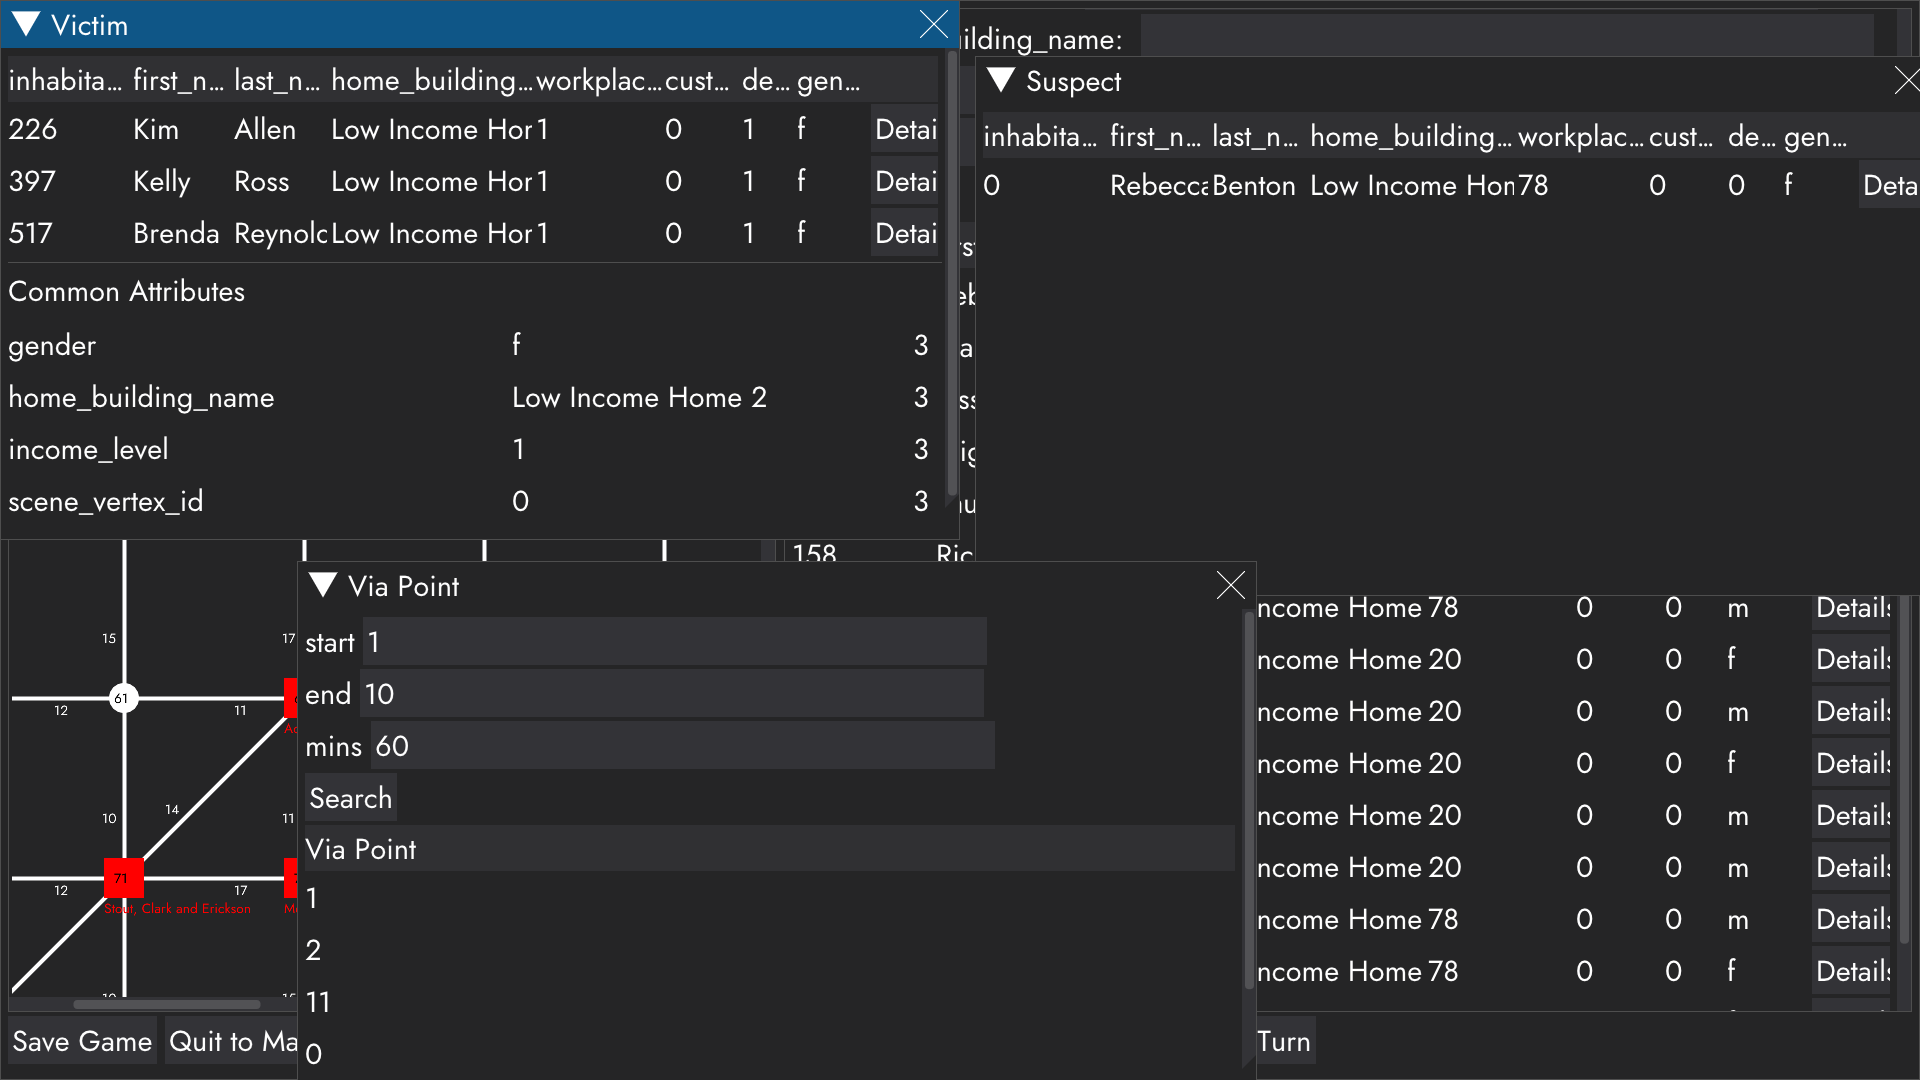
\includegraphics[width=1\textwidth]{victim_suspect_via_point.png}
  \caption{Victim Window, Suspect Window, and Via Point Window.}
  \label{fig:victim_suspect_via_point}
\end{figure}

\begin{figure}[H]
  \centering
  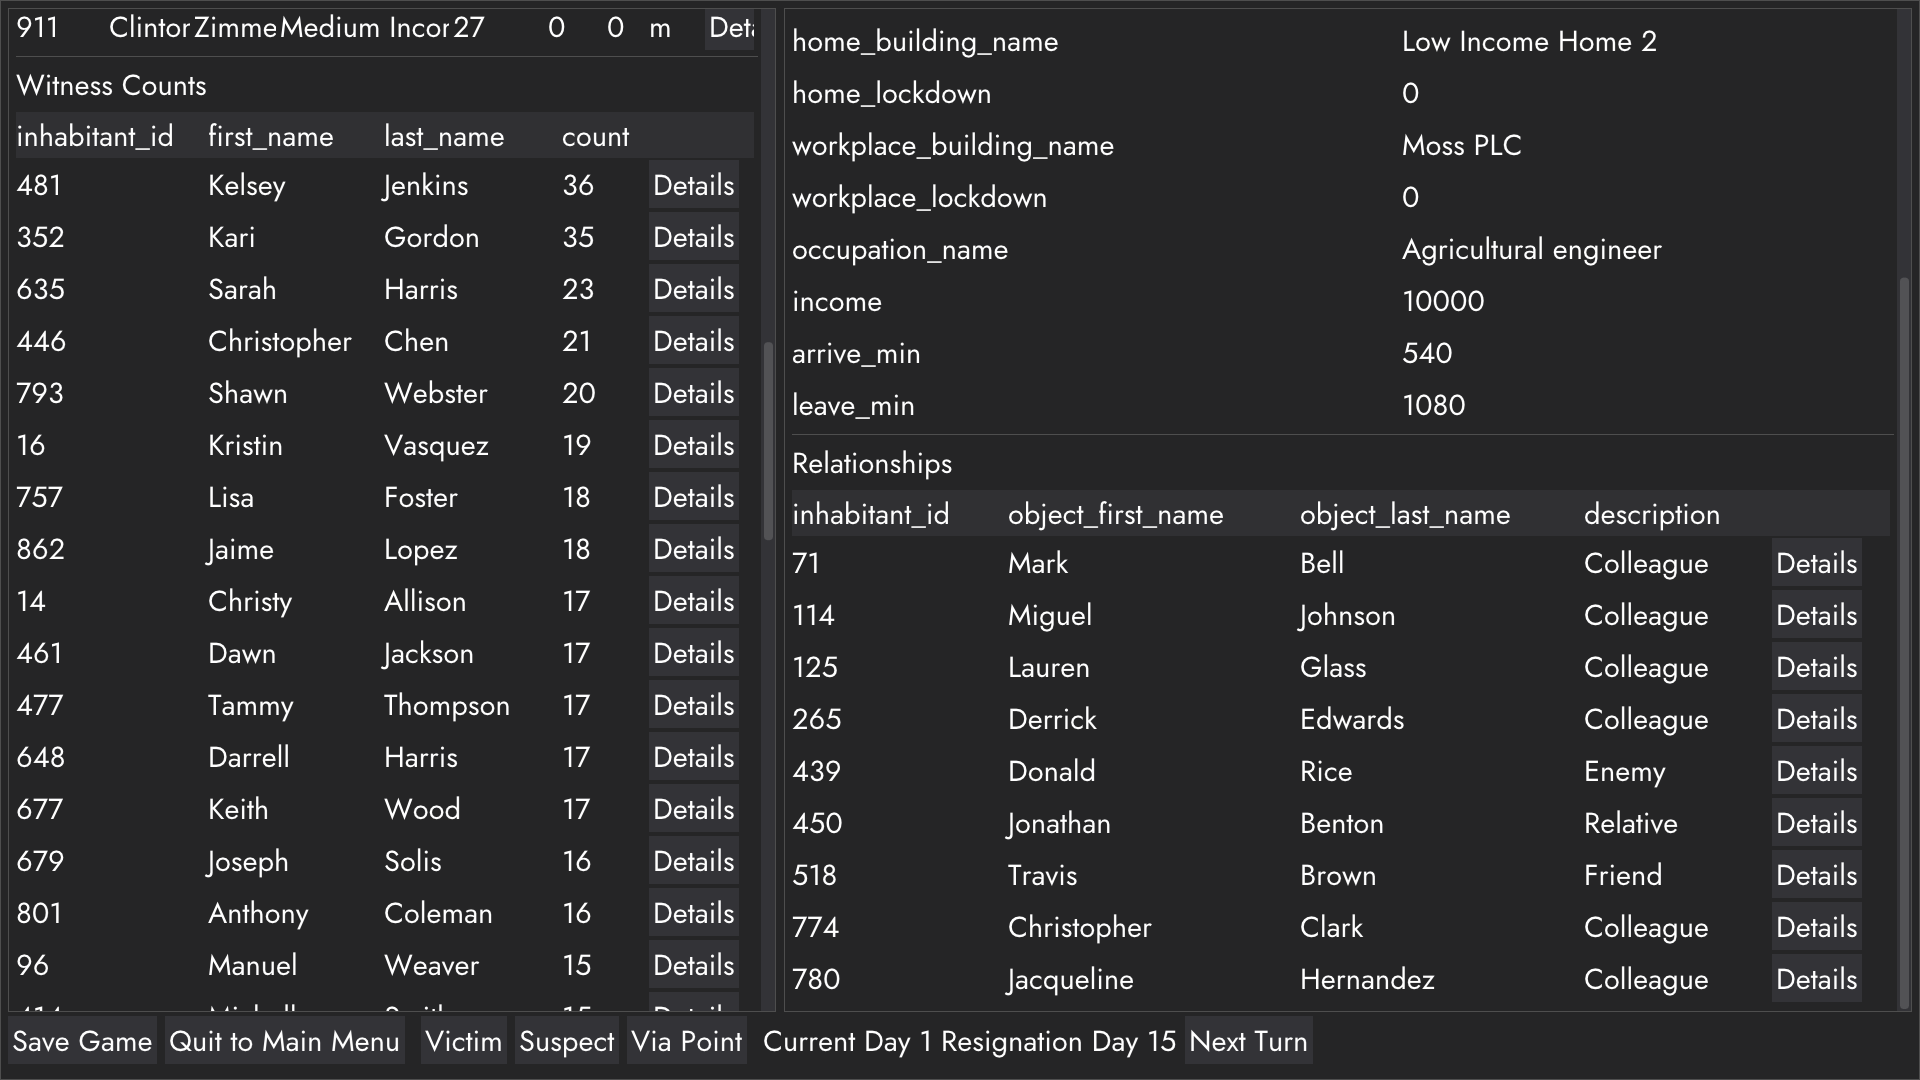
\includegraphics[width=1\textwidth]{witness_counts_relationships.png}
  \caption{Witness Counts and Relationships query.}
  \label{fig:witness_counts_relationships}
\end{figure}

\subsection{Save Screen}
Finally, as shown in Figure \ref{fig:save_game}, when ``Save Game" is clicked, the user is allowed to save a particular instance of the simulation either by overwriting a previously save instance using ``Overwrite," or save as a new instance using ``New Save."

\begin{figure}[H]
  \centering
  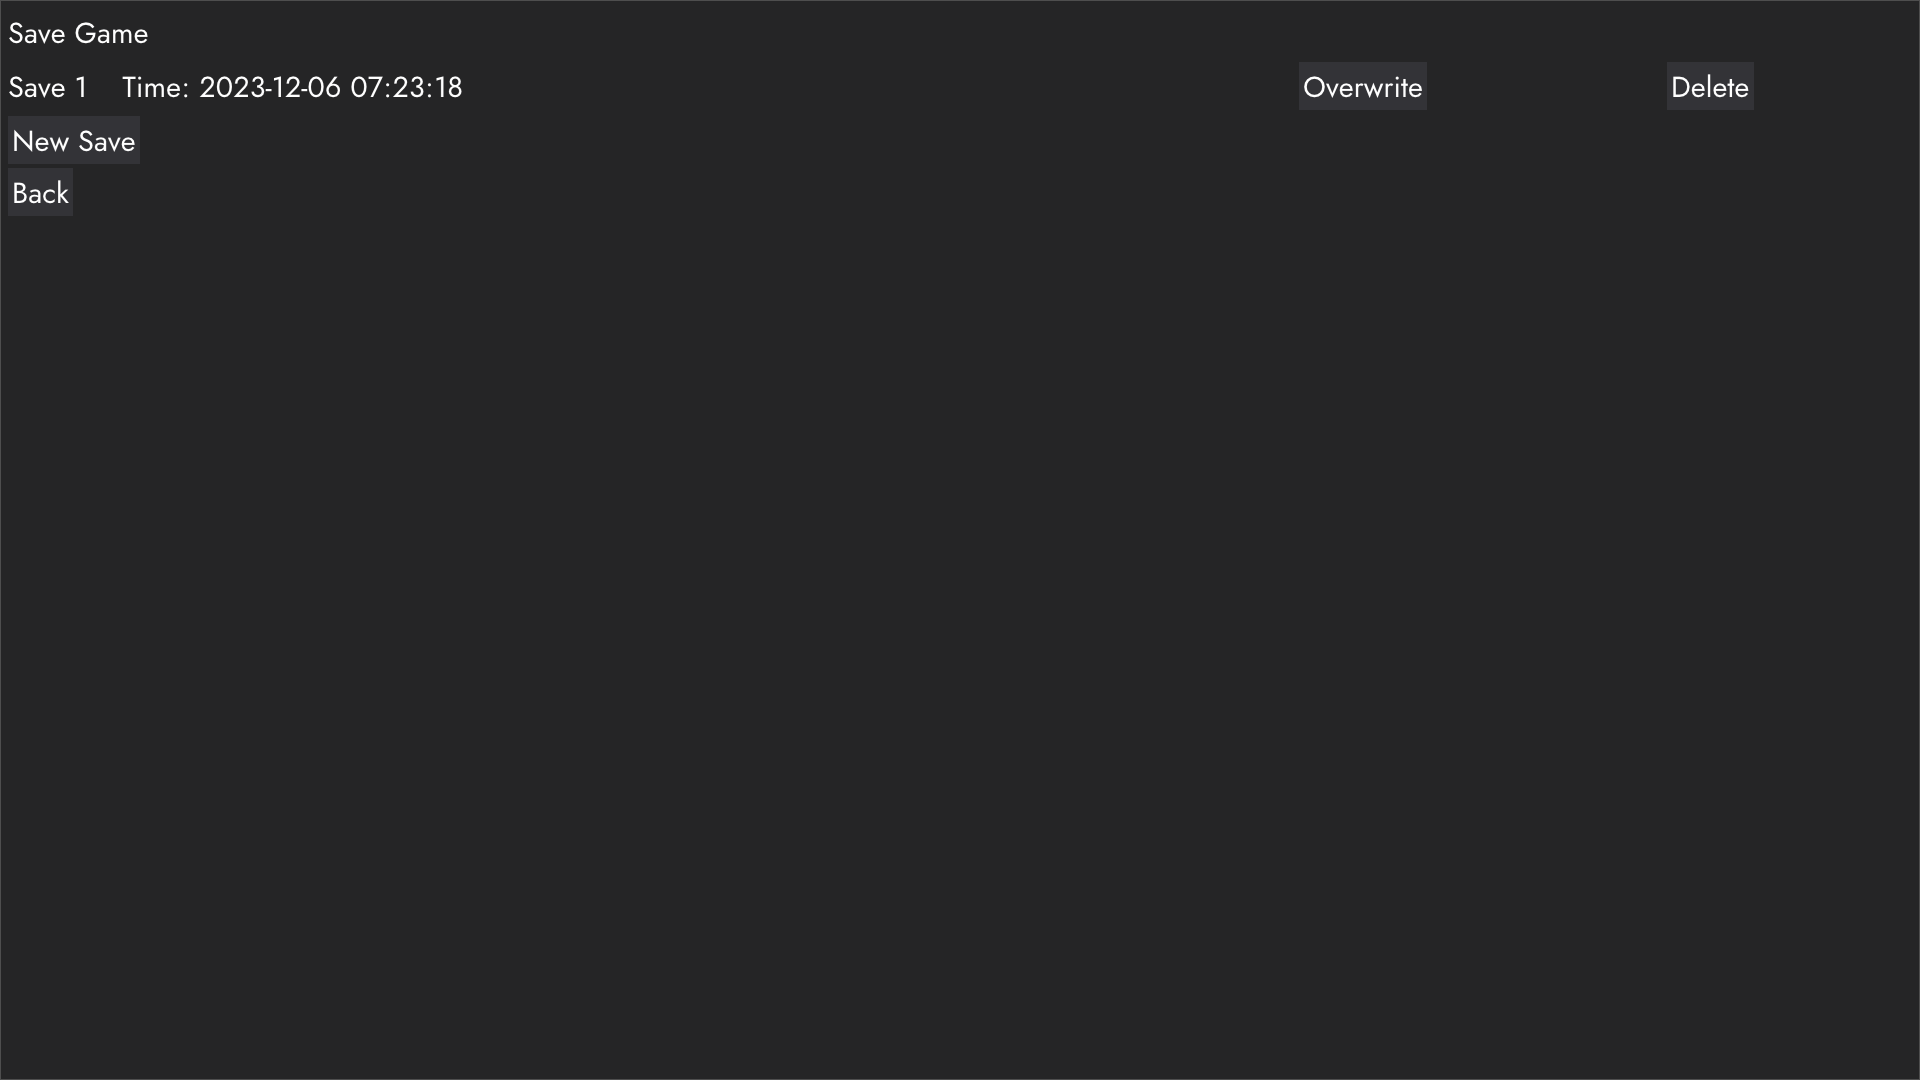
\includegraphics[width=1\textwidth]{save_game.png}
  \caption{Save Screen.}
  \label{fig:save_game}
\end{figure}

\section{Comparison Against Existing Application: SQL Murder Mystery}
The SQL Murder Mystery is an interactive educational tool developed to impart proficiency in Structured Query Language (SQL).\cite{knight_lab_sql_mystery} Originating from the Knight Lab at Northwestern University, this gamified platform engages users in a murder mystery scenario, tasking them with the role of a detective tasked with solving a crime by querying a relational database. While its concept is similar to the project we have created, we believe our simulator offers a much more extensive database and functionality that requires a series of complex queries to implement. It is also noteworthy to mention that the application developed by Knight Lab is geared towards individuals with the purpose of learning introductory SQL queries while our project aims to train the user's deductive skills. This difference can be most explicitly seen from the user interface that our group had developed for the purpose of adding a layer of abstraction to the user.

\section{Conclusion}
The Detective Simulation project successfully encapsulates the intricate aspects of a murder mystery into an immersive game centered around database querying. Through the presented database schema and its refinement process, the structural foundation that enables the game's functionalities is established. Pivotal queries like Path generation and Victim Selection are explored, elucidating the interplay between inhabitants, the murderer, and the overarching simulation environment. These queries constitute the simulation's computational backbone, facilitating intricate behaviors and mirroring real-world complexity.

Additionally, the project demonstrates proficiency in employing recursive triggers to implement complex logic like randomized Path Generation. The use of views to summarize information, as shown by the Victim Commonality example, also reflects an apt utilization of database constructs for analysis.

The graphical user interface, while rudimentary, grants users investigative tools to deduce clues about the murderer's identity. The emulator environment, coupled with the relationship queries, allows methodological tracking of suspects. Saving/loading game states also enables progression over multiple sessions.

Overall, the project presents a comprehensive system melding deductive reasoning and database skills. While scope remains for refinement of UI/UX elements and better feedback to the player after wrong accusations, it stands as a robust foundation readily extensible to more advanced implementations. The work exhibits database design and querying capabilities applicable in both real-world software systems and interactive applications.

\section{Contributions}
\begin{itemize}
    \item Database schema version 1:
    \begin{itemize}
        \item Collective effort amongst Isaac, Yuxiang, and Shanruo
        \item Annotations written by Shanruo
    \end{itemize}
    \item Database schema version 2:
    \begin{itemize}
        \item ER modeling designed by Isaac
        \item Changes to final database schema reflected by Yuxiang
    \end{itemize}
    \item Database data generator:
    \begin{itemize}
        \item building, income\_range, home, occupation and workplace written by Yuxiang
        \item vertex, edge, inhabitant, killer, killer\_chara, status, relationship, victim written by Isaac
    \end{itemize}
    \item Query implementation:
    \begin{itemize}
        \item Shortest path, inhabitant location-time pair generation, witness count, and plausible via point implemented by Yuxiang
        \item Victim selection, victim commonality, inhabitant query implemented by Isaac
        \item Isaac also experimented with implementing the inhabitant location-time pair generation in procedures, which is not used in the final game
    \end{itemize}
    \item Gameplay implementation:
    \begin{itemize}
        \item Simple queries that provide basic information to the users are implemented by both Yuxiang and Isaac
        \item Load-save functionality is written by Yuxiang
        \item Checking the end-game condition and a view for edges that are not blocked is written by Isaac
    \end{itemize}
    \item Front-End UI:
    \begin{itemize}
        \item Individual effort by Yuxiang
    \end{itemize}
\end{itemize}

\pagebreak

\begin{thebibliography}{9}
    \bibitem{sqlite_datatypes}
    SQLite. (2022, April 27). \textit{Datatypes In SQLite}. Retrieved from \url{https://www.sqlite.org/datatype3.html}

    \bibitem{dijkstra_wikipedia}
    Wikipedia. (2023, December 2). \textit{Dijkstra's algorithm}. Retrieved from \url{https://en.wikipedia.org/wiki/Dijkstra%27s_algorithm}
    
    \bibitem{sqlite_forum}
    SQLite Forum. (2021, May 1). \textit{Recursive query to find the shortest path}. Retrieved from \url{https://sqlite.org/forum/info/7c89903050369164}

    \bibitem{dearpygui_github}
    Dear PyGui. (2023). GitHub Repository. Retrieved from \url{https://github.com/hoffstadt/DearPyGui}
\end{thebibliography}

    \begin{thebibliography}{9}
    \bibitem{knight_lab_sql_mystery}
    Knight Lab. (2019). \textit{SQL Murder Mystery}. Retrieved from \url{https://mystery.knightlab.com/}
\end{thebibliography}

\end{document}